\section{Variantendiskussion}
\label{sec:Variantendiskussion}
Zu Beginn soll eine Marktrecherche durchgeführt werden, um bestehende Lösungen zu analysieren und auf Eignung zu Prüfen. Mit den gewonnen Erkenntnissen soll dann abgewägt werden ob Standartsoftware beschafft werden kann oder eine eigenentwicklung Veranlasst wird.

Für die Entwicklung sollen verschidedene Architekturansätze vorgestellt und verglichen werden um so eine Entscheidung für ein vorgehen zu treffen werden das dann im Entwurf und der Implementation Umgesetzt werden kann.
%Das erfolgt im Rahmen einer Variantendiskussion, in der verschiedene Ansätze und Technologien zur Umsetzung der Software bewertet werden.

\subsection{Marktrecherche}
\label{sec:Marktrecherche}
Im Rahmen der Marktrecherche wurden drei verschiedene Softwarelösungen für die Anwesenheitsplanung verglichen. Das Ziel dieser Analyse war es, Akquisitionsoptionen für das geplante Softwareprojekt zu ermitteln. Um Entscheidungen über die Eignung treffen zu können, wurden die Softwareprodukte auf den Erfüllungsgrad ausgewählter Anforderungen geprüft und mit einer Bewertungsmatrix bewertet, die funktionale- und nichtfunktionale Anforderungen beinhaltete. Dabei wurden die Auswahlkriterien so gewählt und gewichtet das zwingend erforderliche Anforderungen höher gewichtet wurden als optionale Anforderungen.

%TODO:Tabelle muss ordentlich Platziert werden
\begin{figure}[htb]
    \centering
    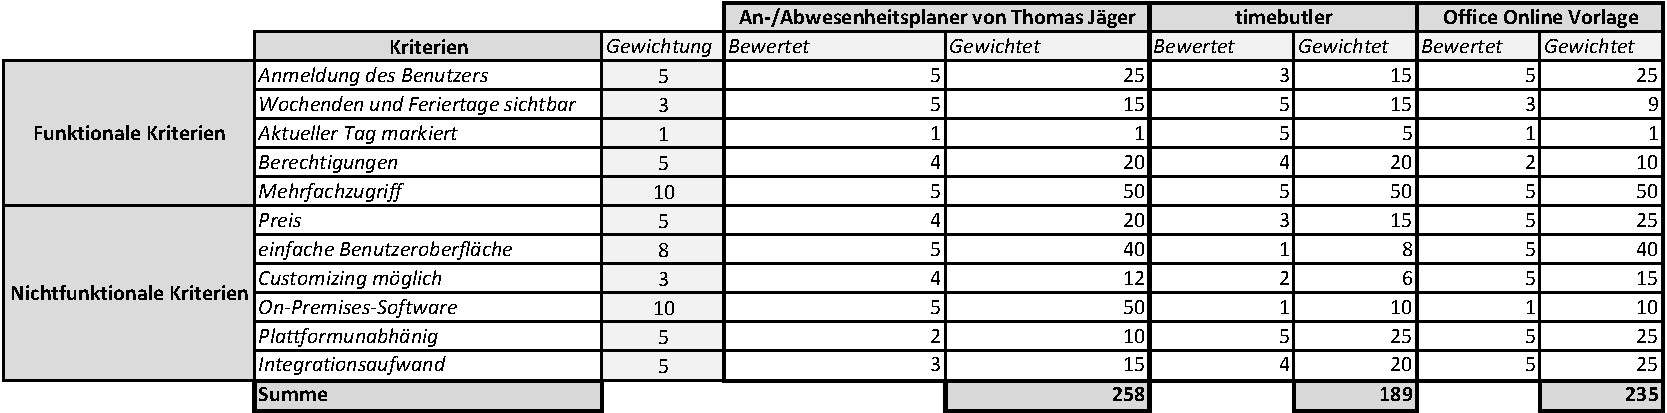
\includegraphics[width=0.9\textwidth,angle=0]{abb/Markterkundung.pdf}
    \caption[Beschreibung]{ Tabelle Markterkundung}
    \label{tab:Markterkundung}
\end{figure}

\subsubsection{An-/Abwesenheitsplaner von Thomas Jäger}
\label{sec:AnAbwesenheitsplaner}
Die erste betrachtete Software, der An-/Abwesenheitsplaner von Thomas Jäger, zeichnete sich durch die besonders intuitive Benutzeroberfläche aus. Bei der Betrachtung der anderen funktionalen Kriterien wurde festgestellt, dass die Software alle benötigten Anforderungen erfüllt und damit für den Einsatz geeignet ist. Negativ zu bewerten ist allerding, das die Software nur als Windows Programm zur Verfügung steht und damit nicht Plattformunabhängig eingesetzt werden kann. Zudem müsste ein solches Programm auf jedem Client PC im SMK installiert werden um die Software für alle Nutzbar zu machen. Damit ergibt sich ein hoher initialer Integrationsaufwand und auch späterer Wartungsaufwand den es zu berücksichtigen gilt. (vgl. \cite{AnAbwesenPlaner})


%Die Benutzerfreundlichkeit wurde jedoch als etwas komplex und steil eingestuft, was eine gewisse Einarbeitungszeit erforderte. Zudem war der Support nur eingeschränkt verfügbar und die Preisgestaltung vergleichsweise hoch. (vgl. \cite{AnAbwesenPlaner})
\subsubsection{timebutler}
\label{sec:timebutler}
Das zweite Programm namens timebutler überzeugte hingegen durch seine Plattformunabhängigkeit. Damit könnte es ohne großen Integrationsaufwand im SMK eingeführt und betrieben werden. Die Software bietet alle geforderten Funktionalitäten hat jedoch eine komplizierte Benutzeroberfläche und stellt viele Funktionen bereit die nicht benötigt werden. Das resultiert in höheren Anschaffungskosten als bei dem An-/Abwesenheitsplaner von Thomas Jäger. Besonders negativ ist zu bewerten, dass die Software zwar Plattformunabhängig ist, da sie auf Webtechnologien aufbaut, jedoch nicht als On-Premises-Software verfügbar ist. Damit müsste auf die Cloud des Anbieters zurückgegriffen werden was nicht gewünscht ist. (vgl. \cite{timebutler})

\subsubsection{Online Office Datei}
\label{sec:OnlineOffice}
Die dritte betrachtete Lösung ist die Verwendung einer Online Tabellenkalkulations Vorlage. Das würde es ermöglichen, die bereits vorhandenen Excel Tabellen für die Anwesenheitsplanung weiter zu verwenden. Durch das zurückgreifen auf Online Funktionalitäten die \zB von Microsoft mit Office356 oder mit Onlyoffice in Verbindung mit Nextcloud zur Verfügung stehen, kann man den gleichzeitigen Zugriff auf diese Listern erreichen. Damit würde man das Hauptproblem der einfachen Excel Dateien lösen. Doch auch hier müsste man im Falle des einsatzes von Office356 auf die Microsoft Cloud zurückgreifen. Desweiteren gibt es nur begrenzte Möglichkeit diese Excel Listen vor ungewollter Änderungen zu schützen und ein Berechtigungskonzept durchzusetzten.

\subsubsection{Auswertung der Marktrecherche}
\label{sec:AuswertungMarktrecherche}
Nach Betrachtung der drei Programme wurde festgestellt, dass keines der drei für eine Akquisition in frage kommt, da jedes seine individuellen Schwachstellen mit sich bringt. Der An-/Abwesenheitsplaner von Thomas Jäger wäre von allen die beste Option, da es eine benutzerfreundliche Oberfläche, eine solide Funktionalität und eine angemessene Preisgestaltung vereint. Die Plattformunabhängigkeit ist jedoch im SMK ein großer Faktor, da sich das neue Programm möglichst gut in die vorhandene Infrastruktur einfügen soll. Deswegen wurde sich gegen eine Akquisition von Standartsoftware entschieden. Um die geforderten Funktionalitäten abzubilden ohne dabei die Schwachstellen der Analysierten Programme inkauf nehmen zu müssen wurde ich für eine Eigenentwicklung der Software entschieden.

\subsection{Eigenentwicklung}
\label{sec:Eigenentwicklung}
Für die Umsetzung wurde Referat 12 mit der Entwicklung der Softwarelösung beauftragt. Die benötigten Hard- und Softwareressourcen vom SMK bereitgestellt und der zeitliche Rahmen für das Projekt wurde mit 32 Arbeitstagen angesetzt. Die genaue Aufschlüsselung des Projektablaufes siehe \ref{abb:Gantt}.

Für die Entwicklung der Software sethen dem Entwickler ein voll ausgestatteter Arbeitsplatz, sowie mehrere virtuelle Maschinen im Rechenzentrum zur Verfügung. Damit hat der Entwickler freie Hand bei der Umsetzung. Zu beachten ist jedoch, dass nach Möglichkeit auf die bestehende Infrastruktur zurückgegriffen bzw. berücksichtigt wird.


\subsection{Umsetzungsvarianten}
\label{sec:Umsetzungsvarianten}
Nach eingehender Analyse der Anforderungen und der Markterkundung wurden verschiedene Umsetzungsvarianten für das geplante Softwareprojekt des Anwesenheitsplaners untersucht. Dabei wurden insbesondere zwei Ansätze für die Entwicklung betrachtet: die monolithische Anwendung und eine Client-Server-Anwendung. Dabei handelt es sich um verschiedene Architekturen mit Vor- und Nachteilen. Architekturen sind in der Softwareentwicklung nicht unbedingt einheitlich Definiert weshalb in den folgenden Absätzen eine gemischte Betrachtung aus der System- und Software Architektur durchgeführt wird. Zusätzlich soll auch auf praktische Umsetzungsvarianten der einzelnen Architekturen eingegangen werden um ein praktisches Beispiel zu geben.

Es soll noch keine Betrachtung des Software Design Patterns angestellt werden, da dieses für den Auswahlprozess der Plattform noch keine Rolle spielt. Dementsprechen wird bei der bergachtung nur erwogen welchen Systemansatz man für die Umsetzung des Projektes wählen sollte.
%Es Softwararchitektur ist vielseitig ...Webbasiert ... Systemarchitektur... Disigneentscheidungen mvvm...

\subsubsection{monolithische Architektur}
\label{sec:monolithisch}
%TODO:was ist monolitisch
Die historisch klassische Form ist die monolithische Architektur. Beim dieser entsteht eine eigenständige Anwendung, die \zB direkt auf den Client PCs installiert wird. Bei diesem Ansatz ist die Software in der Lage, alle erforderlichen Komponenten und Dienste selbst bereitzustellen. Das ist vor allem dann geeignet, wenn die Anwendung auf einer spezifischen Plattform ausgeführt werden soll und keine Notwendigkeit für eine verteilte Architektur besteht. Da die monolithische Architektur sowohl das User-Interface als auch die Logik in einem Prozess beinhaltet, entfällt der zusätzliche Bedarf an einem dedizierten Server zum bearbeiten der Logik. Nachteil hierbei ist die eingeschränkte Flexibilität, da ein solches Programm an das System gebunden ist für das es Entwickelt wurde.

\subsubsection{Client-Server-Architektur}
\label{sec:ClientServer}
%TODO:Was ist Clien-Server
Die zweite betrachtete Option war die Client-Server-Architektur, die bei webbasierten Anwendungen mit einem Backend-Server und einer Datenbank zum Einsatz kommt. Bei dieser Architektur werden die Funktionen auf mehrere Schichten aufgeteilt. Der Backend-Server ist für die Verarbeitung der Anfragen und die Bereitstellung von Daten zuständig, während die Datenbank die persistente Speicherung der Daten ermöglicht. Der Benutzer interagiert mit der Software über das Frontend, das auf dem Client läuft. Um eine Verbindung zwischen Frontend und Backend herzustellen sendet der Client Anfragen an den Server und erwartet entsprechende Antworten mit Daten. Die Kommunikation zwischen Client und Server erfolgt dann über ein Netzwerkprotokoll wie HTTP. Ein Nachteil ist dabei die ständige Netzwerkabhängigkeit der Clients um den Dienst Nutzen zu können und eine erhöhtes maß an Komplexität in der Entwicklung gegenüber der monolithische Architektur.

Als weiterentwicklung der Client-Server-Architektur kommen auch noch die Service Orientierte Architektur (SOA) und die Micro Service Architektur in frage. Diese beiden Architekturansätze erlauben das Backend in kleinere einzeldienste zu zerlegen die dann unabhängig voneinander entwickelt, betrieben und skaliert werden können. Das ist ein großer Vorteil bei besonders großen Projekten in denen verschiedene Technologien und Programmiersprechen eingesetzt werden oder ein sehr hohes Maß an Lastverteilung gefordert ist. Für Projekte mit mittel bis kleinem Umfang ist eine solche Architektur jedoch nicht optimal, da das level an Komplexität extrem steigt und die Vorteile der Architekturen warscheinlicht nicht ausgeschöpft werden können.

\subsubsection{Vergleich}
\label{sec:Vergleich}
Beide der Architekturansätze könnten für den Anwesenheitsplaner eingesetzt werden. Der monolithische Ansatz würde in eine Anwendung für die Windows Clients im SMK münden. Die Software könnte dann als eine Windows Forms oder WPF (Windows Presentation Foundation) Anwendung erstellt werden, was den Vorteil hätte das die Logik und die GUI direkt miteinander verbunden wären und so ein direkter Zugriff auf Benutzereingaben während der Laufzeit möglich ist. Ein weiterer Vorteil ist, dass schon viele Kenntnisse bei der Csharp und Windows Forms Entwicklung vorhanden sind. (vgl. \cite{wpf}, \cite{modernApp})

Eine Client-Server-Architektur in Hinsicht auf eine Browserbasierte Bereitstellung bietet sich ebenfalls an. Die Vorteile eines Webbasierten Ansatzes sind ein sehr hohes Maß an Flexibilität bei den Zielplattformen der Clients und damit eine hohe Zukunftssicherheit. Im Kontext des Projektes des Anwesenheitsplaners bedeutet das, dass der Anwesenheitsplaner auf jedem Gerät im SMK aufgerufen werden kann. Das ist ein wichtiger Faktor, da viele Bedienstete mit moblien Geräten wie Smartphones und Tablets ausgestattet sind. Webbasierte Anwendungen müssen im gegensatz zu Desktop Entwicklungen wie Windows Programmen oder Smartphone Apps nicht installiert werden, das diese von einem zentralen Server bereitgestellt werden und nur von Browser angezeigt werden.

Negative Punkte bei einer Client-Server-Architektur gerade bei Betrachtung von Webtechnologien die erheblich steigende Komplexität. Durch die Trennung von Frontend und Backend muss eine Möglichkeit zur Kommunikation über Schnittstellen geschaffen werden. Das sorgt für eine eingeschränkte Interaktion des Nutzers mit der Logik was zu schlechterer Leistung von Webanwendungen im Vergleich zu Decktopanwendungen führen kann. Um diese Nachteile auszugleichen sollten moderne Frameworks für die Webentwicklung eingesetzt werden. Im Bereich der Webentwicklung ist der Kenntnisstand der Entwickler etwas geringer als bei Decktopanwendungen, was für die Umsetzung Verzögerungen bedeuten könnte. Es sollte also bei diesem Ansatz ein möglichst vertrautes Framework für die Entwicklung verwendet werden.

\subsubsection{Entscheidung}
\label{sec:Entscheidung}
Nach sorgfältiger Abwägung der Vor- und Nachteile beider Ansätze wurde beschlossen, auf eine Client-Server-Architektur mit einer Website als Frontend und einem Webserver als Backend zu setzen um so die Plattformunabhängigkeit von Webtechnologien nutzen zu können. Insgesamt bietet die gewählte Architektur die besten Voraussetzungen für die Umsetzung des Anwesenheitsplaners. Durch eine Webentwicklung wird eine flexible, plattformunabhängige Anwendung geschaffen, die sowohl auf Desktop PCs als auch auf mobilen Geräten und Virtuellen Citrix Maschinen genutzt werden kann ohne neue installationen vornehmen zu müssen.




